\lecture{26}
\title{Recursive Types}
\date{25 April 2016}

\maketitle

\section{Introduction}

Many programming languages have the ability to define recursive data types. For example, suppose we want to define binary trees with integer data at the nodes. In Java we can write
\begin{small}
\begin{alltt}
   class Tree \{
     Tree leftChild, rightChild;
     int data;
   \}
\end{alltt}
\end{small}
A binary tree is an object of this class. In OCaml we can write
\begin{small}
\begin{alltt}
   type tree = Leaf | Node of tree * tree * int
\end{alltt}
\end{small}
These types are _recursive_ because they are defined in terms of themselves.

In the typed \lamcal, we do not yet have any mechanism to define recursive types. We would like the type "tree" to satisfy
\begin{align}
"tree" &= "1 + tree * tree * int",\label{eqn:rec0}
\end{align}
where "1" (aka "unit") represents the empty tree; in other words, we would like the set of data objects inhabiting the type "tree" to be a solution of the equation
\begin{align}
\alpha &= "1 + \alpha * \alpha * int".\label{eqn:rec1}
\end{align}
However, no such solution exists among the types we have seen so far.

How might we augment our type system to include solutions to recursive type equations such as \eqref{eqn:rec1}? There are two basic approaches, called the _equirecursive_ and _isorecursive_ approach, respectively.

\section{Recursive Types as Regular Labeled Trees---The Equirecursive View}

By unwinding \eqref{eqn:rec1}, we can see that
\begin{align*}
\alpha\ &=\ "1" + \alpha * \alpha * "int"\\
&=\ "1" + ("1" + \alpha * \alpha * "int") * ("1" + \alpha * \alpha * "int") * "int"\\
&=\ "1" + ("1" + ("1" + \alpha * \alpha * "int") * ("1" + \alpha * \alpha * "int") * "int") * ("1" + ("1" + \alpha * \alpha * "int") * ("1" + \alpha * \alpha * "int") * "int") * "int"\\
&=\ \cdots
\end{align*}
At each level, we have a finite type with the type variable $\alpha$ appearing at some of the leaves, and we obtain the next level by substituting the right-hand side of \eqref{eqn:rec1} for $\alpha$. This gives a sequence of deeper and deeper finite trees, where each successive tree is a substitution instance of the previous tree.

If we take the limit of this process, we have an infinite tree. We can think of this as an infinite labeled graph whose nodes are labeled with the type constructors *, +, "int", and "1". This is very much like an ordinary type expression, except that it is infinite. There are no more $\alpha$'s, because we have substituted for all of them all the way down. This infinite tree is a solution of \eqref{eqn:rec1}, and this is what we take as the type "tree".

In general, let $\Sigma$ be a signature consisting of several type constructors of various arities. For example, $\Sigma$ might consist of the type constructors $\to$, "*", "+", "1", and "int". We can form the set of (finite) types over $\Sigma$ inductively in the usual way. Each such type can be regarded as a finite labeled tree. For example, the type $"int" \to "int" \to "int"$ can be viewed as the labeled tree
\begin{center}
 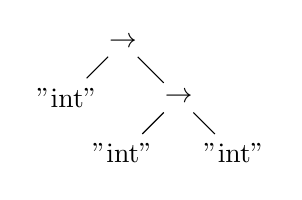
\begin{tikzpicture}[node distance=1cm]
  \node (0) {$\to$};
  \node (1) [below left of=0] {"int"};
  \node (2) [below right of=0] {$\to$};
  \node (3) [below left of=2] {"int"};
  \node (4) [below right of=2] {"int"};
  \draw (0) -- (1);
  \draw (0) -- (2);
  \draw (2) -- (3);
  \draw (2) -- (4);
 \end{tikzpicture}
\end{center}
Now let us add some infinite types. These are infinite labeled trees that respect the arities of the constructors in $\Sigma$; that is, if the constructor is binary (such as "*" or $\to$), any node labeled with that constructor must have exactly two children; and if the constructor is nullary, such at "1", then any node labeled with that symbol must be a leaf. Within these constraints, the tree may be infinite.\footnote{For a more formal account of this construction, see Handout 2A, \S1.2 (27 January).}

A (finite or infinite) expression with only finitely many subexpressions up to isomorphism is called _regular_. For example, the infinite type
\begin{center}
 \begin{tikzpicture}[node distance=1cm]
  \node (0) {$\to$};
  \node (1) [below left of=0] {"int"};
  \node (2) [below right of=0] {$\to$};
  \node (3) [below left of=2] {"int"};
  \node (4) [below right of=2] {$\to$};
  \node (5) [below left of=4] {"int"};
  \node (6) [below right of=4, node distance=12mm] {$\ddots$};
  \draw (0) -- (1);
  \draw (0) -- (2);
  \draw (2) -- (3);
  \draw (2) -- (4);
  \draw (4) -- (5);
  \draw (4) -- (6);
 \end{tikzpicture}
\end{center}
is regular, since it has only two subexpressions up to isomorphism, namely itself and "int". The limit of the unwinding of \eqref{eqn:rec1} above, which we took to be the type "tree", is also regular; it has exactly five subexpressions up to isomorphism, namely "tree", "1", "tree * tree * int", "tree * tree", and "int".

Regular trees are all we need to provide solutions to finite systems of type equations of the form \eqref{eqn:rec1}. Suppose we have $n$ type equations in $n$ variables:
%\begin{align}
%\alpha_1 &= \tau_1\nonumber\\
%& \vdots\label{eqn:rec3}\\
%\alpha_n &= \tau_n,\nonumber
%\end{align}
\begin{align}
\alpha_1 &= \tau_1,\ \ldots,\ \alpha_n = \tau_n\label{eqn:rec3}
\end{align}
where each $\tau_i$ is a finite type over the type constructors $\Sigma$ and type variables $\seq\alpha 1n$. This system has a solution $\seq\sigma 1n$ in which each $\sigma_i$ is a regular tree. Moreover, if no right-hand side is a variable, then the solution is unique.

\subsection{The $\mu$ Constructor}

We can specify the infinite solutions to systems of type equations \eqref{eqn:rec3} using a finite syntax involving a new type constructor $\mu$, the _fixpoint type constructor_. If we have an equation $\alpha = \tau$ such that the right-hand side is not $\alpha$, then there is a unique solution, which is a finite or infinite regular tree. The solution will be infinite if $\alpha$ occurs in $\tau$ and will be finite (in fact it will just be $\tau$) if $\alpha$ does not occur in $\tau$. We denote this unique solution by $\mut\alpha\tau$.

Syntactically, $\mu$ acts as a binding operator in type expressions as $\lambda$ does in $\lambda$-terms, with the same notions of scope, free and bound variables, $\alpha$-conversion, and safe substitution.

Since $\mut\alpha\tau$ is a solution to $\alpha=\tau$, we have
\begin{align}
\mut\alpha\tau &= \subst\tau{\mut\alpha\tau}\alpha.\label{eqn:rec2}
\end{align}

For example, to get a "tree" type satisfying \eqref{eqn:rec0}, we can define
\begin{align*}
"tree"\ &\definedas\ \mut\alpha{"1 + \alpha * \alpha * int"}.
\end{align*}
The desired equation \eqref{eqn:rec0} is just \eqref{eqn:rec2} for this case.

The solutions $\seq\sigma 1n$ to any finite system of the form \eqref{eqn:rec3} can be expressed in terms of $\mu$. For example, suppose $\tau_1$ and $\tau_2$ are finite type expressions over the type variables $\alpha_1,\alpha_2$ such that neither $\tau_1$ nor $\tau_2$ is a variable. The system
\begin{align*}
\alpha_1 &= \tau_1 & \alpha_2 &= \tau_2
\end{align*}
has a unique solution $\sigma_1,\sigma_2$ specified by
\begin{align*}
\sigma_1 &= \mut{\alpha_1}{(\subst{\tau_1}{\mut{\alpha_2}{\tau_2}}{\alpha_2})} &
\sigma_2 &= \mut{\alpha_2}{(\subst{\tau_2}{\mut{\alpha_1}{\tau_1}}{\alpha_1})}.
\end{align*}

Mutually recursive type declarations arise quite often in practice. For example, consider the following Java class definitions:
\begin{small}
\begin{alltt}
   class Node \{
     Edge[] inEdges, outEdges;
   \}
   class Edge \{
     Node source, sink;
   \}
\end{alltt}
\end{small}
Note that \texttt{Node} refers to \texttt{Edge} and vice versa. So we must take a mutual fixpoint when assigning types.

\subsection{Typing Rules}

In the equirecursive view, since $\mut\alpha\tau=\subst\tau{\mut\alpha\tau}\alpha$, the typing rules are quite simple:
\begin{align*}
\AxiomC{$\Gjudge e{\subst\tau{\mut\alpha\tau}\alpha}$}
\RightLabel{($\mu$-intro)}
\UnaryInfC{$\Gjudge e{\mut\alpha\tau}$}
\DisplayProof
&&
\AxiomC{$\Gjudge e{\mut\alpha\tau}$}
\RightLabel{($\mu$-elim)}
\UnaryInfC{$\Gjudge e{\subst\tau{\mut\alpha\tau}\alpha}$}
\DisplayProof
\end{align*}
%\[
%\begin{array}{c@{\qquad\qquad}c}
%\mbox{($\mu$-intro)} \quad \linfer{\Gjudge e{\mut\alpha\tau}}{\Gjudge e{\subst\tau{\mut\alpha\tau}\alpha}}
%&
%\mbox{($\mu$-elim)} \quad \linfer{\Gjudge e{\subst\tau{\mut\alpha\tau}\alpha}}{\Gjudge e{\mut\alpha\tau}}
%\end{array}
%\]
Equivalently, we can just allow substitution of equals for equals in type expressions.

\section{Folding and Unfolding---The Isorecursive View}

There is another approach to recursive types, the _isorecursive_ approach. Here we do not have any infinite types, but rather the expression $\mut\alpha\tau$ is itself a type. In this approach, $\mut\alpha\tau$ and $\subst\tau{\mut\alpha\tau}\alpha$ are considered different (but isomorphic) types. 

The step of substituting $\mut\alpha\tau$ for $\alpha$ in $\tau$ is called _unfolding_, and the reverse operation is called _folding_. The conversion of elements between these two types is accomplished by explicit "fold" and "unfold" operations.
\begin{align*}
"unfold"_{\mut\alpha\tau} &: \mut\alpha\tau\ \to\ \subst\tau{\mut\alpha\tau}\alpha
&
"fold"_{\mut\alpha\tau} &: \subst\tau{\mut\alpha\tau}\alpha\ \to\ \mut\alpha\tau
\end{align*}
(we suppress the subscripts when there is no ambiguity). In this view, the equality symbol in \eqref{eqn:rec2} is not really an equality, but just an isomorphism.

\subsection{Typing Rules}

In the isorecursive view, the typing rules consist of a pair of introduction and elimination rules for $\mu$-types that explicitly mention "fold" and "unfold":
\begin{align*}
\AxiomC{$\Gjudge e{\subst\tau{\mut\alpha\tau}\alpha}$}
\RightLabel{($\mu$-intro)}
\UnaryInfC{$\Gjudge{"fold"~e}{\mut\alpha\tau}$}
\DisplayProof
&&
\AxiomC{$\Gjudge e{\mut\alpha\tau}$}
\RightLabel{($\mu$-elim)}
\UnaryInfC{$\Gjudge{"unfold"~e}{\subst\tau{\mut\alpha\tau}\alpha}$}
\DisplayProof
\end{align*}
%\[
%\begin{array}{c@{\qquad\qquad}c}
%\mbox{($\mu$-intro)} \quad \linfer{\Gjudge{"fold"~e}{\mut\alpha\tau}}{\Gjudge e{\subst\tau{\mut\alpha\tau}\alpha}}
%&
%\mbox{($\mu$-elim)} \quad \linfer{\Gjudge{"unfold"~e}{\subst\tau{\mut\alpha\tau}\alpha}}{\Gjudge e{\mut\alpha\tau}}
%\end{array}
%\]

\subsection{Structural Operational Semantics}

In the isorecursive view, we also need to augment the operational semantics. We only need one rule:
\begin{align*}
"unfold"~("fold"~e)\ &\to\ e.
\end{align*}
Intuitively, to access the data in a recursive type $\mut\alpha\tau$, we need to unfold it first; but the only way that values of type $\mut\alpha\tau$ could have been created in the first place is via a "fold".

\subsection{An Example}

Suppose we want to write a program to add a list of numbers. The list type is a recursive type, which we can define as
\begin{align*}
"intlist"\ &\definedas\ \mut\alpha{"1 + int * \alpha"}.
\end{align*}
The type "1" (aka "unit") represents the empty list. It has a single inhabitant "null". The other case is for a nonempty list consisting of a head, which is an "int", followed by the tail of the list, which is an "intlist"; that is, "int * intlist".

Now we can write a function "sum" to add up an "intlist". This will be a recursive function, so we will need to take a fixpoint.
\[
\letin{"sum"}{"rec"~f : "intlist" \arrow "int" .\, \lam{\ell : "intlist"}{\ldots}}{\ldots}
\]
In the body of this function, we would like to do a "match" on the "intlist" $\ell$. But to do a "match", we need a sum type, and $\ell$ is a $\mu$-type, so we will have to unfold it first. So the body would be
\[
\begin{array}l
"match"~"unfold"~\ell:"1 + int * intlist"~"with"\\
\phantom{dd}|\ \lam{u:"1"}0\\
\phantom{dd}|\ \lam{p:"int * intlist"}{("fst"~p) + f\,("snd"~p)}
\end{array}
\]
This is just the same code that you would write in OCaml, except we have explicitly shown the recursion in the definition of the "intlist" type and the "unfold" that is needed to get the exploded view of the type.

\section{Equirecursive vs Isorecursive}

Programming languages deal with recursive types in different ways. Java, Modula-3, and OCaml take the equirecursive approach, in which the folded and unfolded types are considered equal, and the "fold"/"unfold" operations are just the identity functions. Recursive types and their unfoldings are fully substitutable for each other. 
\begin{small}
\begin{alltt}
   class E \{
     String x;
     E e;
     public String toString() \{
       return e.e.e.e.e.e.e.e.e.e.e.e.e.e.e.e.x;
     \}
   \}
\end{alltt}
\end{small}
On the other hand, CLU, and C use isorecursive types, in which $\mut\alpha\tau$ and $\subst\tau{\mut\alpha\tau}\alpha$ are considered different (but isomorphic) types, and the casting operators "fold" and "unfold" are required to go between them. CLU uses "up" and "down" instead of "fold" and "unfold".
%In OCaml, the "unfold" operator is performed automatically and implicitly by the "match" and "let" statements and the pattern-matching mechanism. The type constructors in a recursive datatype definition, applied to arguments, act as "fold" operations.
%\begin{small}
%\begin{alltt}
%   \# type tree = Leaf | Node of tree * tree * int;;
%   type tree = Leaf | Node of tree * tree * int
%   \# Node (Leaf, Leaf, 4);;
%   - : tree = Node (Leaf, Leaf, 4)
%\end{alltt}
%\end{small}

\section{Numbers as a Recursive Type}

We started with primitive types "1", "boolean", and "int". We have already seen that the type "boolean" can be represented as "1 + 1" with values "false" and "true" represented by "inL null" and "inR null", respectively.

Now that we have recursive types, we no longer need to take "int" as primitive, but we can define it as a recursive type. A natural number is either $0$ or a successor of a natural number. Thus we can take
\begin{align*}
"nat" &\definedas \mut\alpha{"1" + \alpha} &
"0" &\definedas "fold~(inL~null)" &
"1" &\definedas "fold~(inR~0)" &
"2" &\definedas "fold~(inR~1)",
\end{align*}
and so on. Here $"fold" = "fold"_{"nat"}$, $"inL" = "inL"_{"1+nat"}$, and $"inR" = "inR"_{"1+nat"}$.

We can use the recursive type "nat" to code up all of the usual arithmetic, and all these operations are well-typed. For example, the successor function would be
\[
(\lam{x : "nat"}{"fold"~("inR"~x)}) : "nat \to nat".
\]
So all we really need as primitive types and type constructors are "1" ("unit"), recursive types, products, and sums, and of course $\to$. With these we can build all the other types like natural numbers, integers, lists, trees, floating point numbers, and so on.

\section{Self-Application and $\Omega$}

Recall the _paradoxical combinator_ $\Omega$ defined by
\begin{align*}
\omega &\definedas \lam{x}{xx} &
\Omega &\definedas \omega\omega.
\end{align*}
We can now give these terms recursive types, provided we insert some folding and unfolding. Since $x$ is applied as a function, it must have some kind of function type, say $\sigma\to\tau$. But since it is applied to itself as an argument, it must also have type $\sigma$. This seems to indicate that the type of $x$ must satisfy the equation $\sigma=\sigma\to\tau$. The recursive type $\mut\alpha{(\alpha\to\tau)}$ appears to be in order (here $\tau$ can be anything).

To actually apply $x$ to $x$, we have to unfold it. The type of $"unfold"~x$ is
\begin{align*}
"unfold"~x : (\mut\alpha{(\alpha\to\tau)})\ &\to\ \tau.
\end{align*}
This is a function with domain $\mut\alpha{(\alpha\to\tau)}$, which is the type of $x$, so we can apply it to $x$. The type of the result $("unfold"~x)~x$ is $\tau$. Thus the fully typed $\omega$ term is
\begin{align*}
\omega\ &\definedas\ (\lam{x : \mut\alpha{(\alpha\to\tau)}}{("unfold"~x)~x}) : (\mut\alpha{(\alpha\to\tau)})\to\tau.
\end{align*}

If we now fold this, we get
\[
"fold"~\omega : \mut\alpha{(\alpha\to\tau)}.
\]
Therefore, we can apply $\omega$ as a function to $"fold"~\omega$, and the result is
\[
\omega~("fold"~\omega) : \tau.
\]
This is the same as the original $\Omega$ term, but with explicit folding and unfolding.

We can do this in OCaml:
\begin{small}
\begin{alltt}
   \# type u = Fold of (u -> u);;
   type u = Fold of (u -> u)
   \# let omega = fun x -> match x with Fold f -> f x;;
   val omega : u -> u = <fun>
   \# omega (Fold omega);;
\end{alltt}
\end{small}
%\begin{code}
%\tt
%  \# type u = Fold of (u -> u);;
%  type u = Fold of (u -> u)
%  \# let omega = fun x -> match x with Fold f -> f x;;
%  val omega : u -> u = <fun>
%  \# omega (Fold omega);;
%\end{code}
(\textit{and at this point it will just sit there forever until you hit control-c})
\begin{small}
\begin{alltt}
   {\caret}CInterrupted.
\end{alltt}
\end{small}
%\begin{code}
%\tt
%  $\caret$CInterrupted.
%\end{code}
So we were finally able to introduce nontermination. But the point is that it passed typechecking, so the program was well-typed.

\section{Untyped to Typed $\lambda$-Calculus}

With recursive types, we can type everything in the pure untyped \lamcal. Every $\lambda$-term can be applied as a function to any other $\lambda$-term, so every $\lambda$-term (with appropriate folds and unfolds inserted) has type $U \definedas \mut\alpha{\alpha\to\alpha}$. The translation is
\begin{align*}
\SB[D]x\ &\definedas\ x\\
\SB[D]{e_0\,e_1}\ &\definedas\ ("unfold"~\SB[D]{e_0})~\SB[D]{e_1}\\
\SB[D]{\lam xe}\ &\definedas\ "fold"~\lam{x:U}{\SB[D]e}.
\end{align*}
Note that every untyped term maps to a term of type $U$.
